\subsection{Synchronous agent interactions}
With the concepts introduced so far we can achieve already a lot in terms of agent interactions: agents can react to incoming events, which are either the \textit{Tick} event advancing simulation time by one step or a message sent by another agent (or the agent itself). This is enough to implement simple one-directional agent interactions where one agent sends a message to another agent but does not await an answer within the same \textit{Tick}. This one-directional interactions is used in the model to implement the passing of diseases, the paying back of debt, passing on wealth to children upon death - the agent simply sends a message and forgets about it.

Unfortunately this mechanism is not enough to implement the other agent-interactions in the Sugarscape model, which are structurally richer: they need to be synchronous. In the use-cases of mating, trading and lending two agents need to come to an agreement over multiple interactions steps within the same \textit{Tick} which need to be exclusive and synchronous.  This means that an agent A initiates such a multi-step conversation with another agent B by sending an initial message to which agent B has to react by a reply to agent A who upon reception of the message, will pick up computation from that point and reply with a new message and so on. Both agents must not interact with other agents during this conversation to guarantee resource constraints, otherwise it would become quite difficult and cumbersome to ensure that agents don't spend more than they have when trading with multiple other agents at the same time. Also the initiating agent A must be able to pick up processing of its \textit{Tick} event from the point where it started the conversation with agent B because sending a message always requires the handling of the current event to exit and hand the control back to the simulation kernel. See Figure \ref{fig:syncagentinteractions} for a visualisation of the sequence of actions.

\begin{figure}
	\centering
	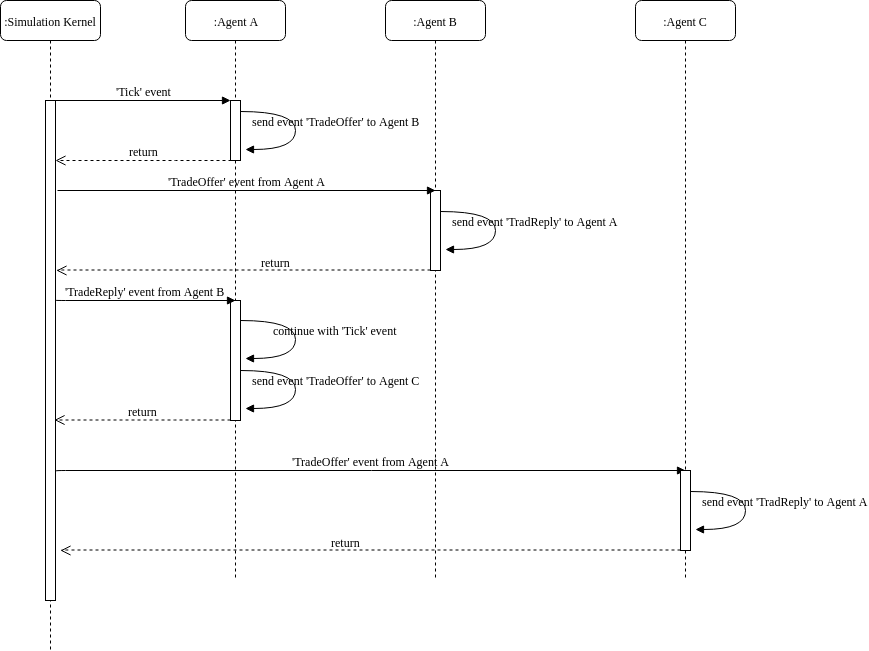
\includegraphics[width=1.0\textwidth, angle=0]{./fig/eventdriven/syncagentinteractions.png}
	\caption{Sequence diagram of synchronous agent interaction in the trading use-case. Upon the handling of the \textit{Tick} event, agent A looks for trading partners and finds agent B within its neighbourhood and sends a \textit{TradingOffer} message. Agent B replies to this message with \textit{TradeReply} and agent A continues with the trading algorithm by picking up where it has left the execution when sending the message to agent B. After agent A has finished the trading with agent B, it turns to agent C, where the same procedure follows.}
	\label{fig:syncagentinteractions}
\end{figure}

The way to implement this is to allow an agent to be able to change its internal event-handling state: to switch into different event-handlers, after having sent an event, to be able to react to the incoming reply in a specific way by encapsulating local state for the current synchronous interaction through closures and currying. Further, by making use of continuations the agent can pick up the processing of the \textit{Tick} event after the synchronous agent interaction has finished. Key to this is the function \textit{continueWithAfter} which we already shortly introduced through \textit{generalEventHandler}. This function takes an MSF which returns an output of type \textit{b} and an optional MSF. If this optional \textit{Maybe} MSF is \textit{Just} then the \textit{next} input is handled by this new MSF. In case no new MSF is returned (\textit{Nothing}), the MSF will stay the same. This is a more specialised version of the \textit{switch} combinator introduced in Chapter \ref{sec:back_frp} in the way that it doesn't need an additional function to produce the actual MSF continuation. Note that the semantics are different though: whereas \textit{switch} runs the new MSF immediately, \textit{continueWithAfter} only applies the new MSF in the \textit{next} step. The implementation of the function is as follows:

\begin{HaskellCode}
continueWithAfter :: Monad m => MSF m a (b, Maybe (MSF m a b)) -> MSF m a b
continueWithAfter msf = MSF (\a -> do
  ((b, msfCont), msf') <- unMSF msf a
  let msfNext = fromMaybe (continueWithAfter msf') msfCont
  return (b, msfNext))
\end{HaskellCode}

Finally, we can discuss the \textit{Tick} handling function. It returns a value of type \textit{Maybe (EventHandler g)} which if is \textit{Just} will result in to a change of the top-level event handler through \textit{continueWithAfter} as shown in \textit{generalEventHandler} above. Note the use of continuations in the case of \textit{agentMating, agentTrade} and  \textit{agentLoan}. All these functions return a \textit{Maybe (EventHandler g)} because all of them can potentially result in synchronous agent interactions which require to change the top-level event handler. The function \textit{agentDisease} is the last in the chain of agent behaviour, thus we are passing a default continuation which simply switches back into \textit{generalEventHandler} to finish the processing of a \textit{Tick} in an agent.

\begin{HaskellCode}
handleTick :: RandomGen g => DTime -> AgentLocalMonad g (Maybe (EventHandler g))
handleTick dt = do
  -- perform ageing of agent
  agentAgeing dt
  -- agent move, returns amount it of resources it harvested
  harvestAmount <- agentMove
  -- metabolise resources, depending on agents metabolism rate
  -- returns amount metabolised
  metabAmount <- agentMetabolism
  -- polute environment given harvest and metabolism amount
  agentPolute harvestAmount metabAmount

  -- check if agent has starved to death or died of age
  ifThenElseM
    (starvedToDeath `orM` dieOfAge)
    (do
      -- died of age or starved to deat: remove from simulation
      agentDies agentMsf
      return Nothing) 
    -- still alive, perform the remaining steps of the behaviour
    -- pass agentContAfterMating as continuation to pick up after mating
    -- synchronous conversations have finished
    (agentMating agentMsf agentContAfterMating)

-- after mating continue with cultural process and trading
agentContAfterMating :: RandomGen g => AgentLocalMonad g (Maybe (EventHandler g))
agentContAfterMating = do
    agentCultureProcess
    -- pass agentContAfterTrading as continuation to pick up after trading 
    -- synchronous conversations have finished
    agentTrade agentContAfterTrading 

-- after trading continue with lending and borrowing
agentContAfterTrading :: RandomGen g  => AgentLocalMonad g (Maybe (EventHandler g))
agentContAfterTrading = agentLoan agentContAfterLoan

-- after lending continue with diseases, which is the step in a Tick event
agentContAfterLoan :: RandomGen g => AgentLocalMonad g (Maybe (EventHandler g))
agentContAfterLoan = agentDisease defaultCont

-- safter diseases imply switch back into the general event handler
defaultCont :: RandomGen g => AgentLocalMonad g (Maybe (EventHandler g))
defaultCont = return (Just generalEventHandler)
\end{HaskellCode}

\subsubsection{Tagless final}
Although the indirect, continuation based approach to synchronous agent interactions as shown before works, it is quite cumbersome, fragile and it is easy to get something wrong. What would be more desirable is to have a truly synchronous approach, where the reply to an event happens directly as a result of the \textit{sendEventTo} function: when calling \textit{sendEventTo}, behind the scenes the receiving agent is executed and the result is returned directly to the caller, without any indirections. With the \textit{tagless final} approach as introduced in the event-driven SIR above, this becomes possible in an elegant and robust way. We have developed this concept for the event-driven SIR only. Still, it should be equally applicable for the Sugarscape but we leave that for further research.

We start by extending the API by defining a \textit{new} typeclass \textit{MonadAgentSync}:

\begin{HaskellCode}
class Monad m => MonadAgentSync e m | m -> e where
  sendSync :: e -> AgentId -> m (Maybe [e])
\end{HaskellCode}

The semantics behind the \textit{sendSync} method shall be that it allows to send an event of type \textit{e} to agent with id \textit{AgentId}. If the agent cannot be found it will return \textit{Nothing}, otherwise it will return \textit{Just} the list of events the receiving agent replies to the sending agent. 

The only place which has to be changed is the susceptible agent but due to the different semantics, parts of its behaviour needs to be rewritten. The receiving agents are left unchanged as at the moment a receiver has no means to distinguish between asynchronous and synchronous events and is not forced to reply to the sender in case of a synchronous event. It would be useful to have some mechanism that in case of a synchronous event, the receiver can only reply to the sender. We leave that issue for further research.

Handling an incoming \textit{Contact} from an \textit{Infected} is no longer necessary as it will not happen, because the interactions go directly through \textit{sendSync} and infected agents don't make contact pro-actively. Thus, the \textit{MakeContact} handler has to be changed to take into account that the infection can happen directly there:

\begin{HaskellCode}
handleEvent MakeContact = do
  ais        <- getAgentIds
  ai         <- getMyId
  isInfected <- makeContact beta ai ais
  if isInfected
    -- got infected, signal event to switch
    then return (Just ())
    else do
      -- not infected, re-schedule MakeContact
      scheduleMakeContact
      return Nothing
\end{HaskellCode}

The function \textit{makeContact} recursively \textit{makeContactWith} $\beta$ (contact rate) other agents. Whereas previously, sending a \textit{Contact} event to itself was not a problem, this is not allowed any more and must be prevented explicitly. The reason for that is discussed below in the implementation of the \textit{sendSync} method of the pure interpreter. Note that sending to itself counts against the $\beta$ contacts, as it would make no difference: receiving a \textit{Contact} from a \textit{Susceptible} has no effect on a susceptible agent anyway. If the case arises in a model that agents need to send events to themselves, it cannot happen through mechanisms like \textit{sendSync} but it has to go through asynchronous scheduling of events which decouples the sending from the receiving.

\begin{HaskellCode}
makeContact :: (MonadAgent SIREvent m, MonadAgentSync SIREvent m)
            => Int       -- ^ number of contacts to make
            -> AgentId   -- ^ sender agent id
            -> [AgentId] -- ^ all agent ids (including self)
            -> m Bool
makeContact 0 _ _ = return False
makeContact n ai ais = do
  receiver <- randomElem ais
  -- prevent sending to self
  if ai == receiver
    -- self counts against beta contacts
    then makeContact (n-1) ai ais
    else do
      -- make contact
      ret <- makeContactWith receiver
      if ret
        -- got infected, stop
        then return True
        -- not infected, continue
        else makeContact (n-1) ai ais
\end{HaskellCode}

Finally we can use \textit{sendSync} to directly send events to a receiving agent, which replies with a list of events to the sender. Note that we needed to add the new \textit{MonadAgentSync} typeclass to the overloaded function, to make the \textit{sendSync} method available.

\begin{HaskellCode}
makeContactWith :: (MonadAgent SIREvent m, MonadAgentSync SIREvent m) 
                => AgentId -> m Bool
makeContactWith receiver = do
  ai     <- getMyId
  -- DIRECT SYNCHRONOUS AGENT INTERACTION HAPPENS HERE
  retMay <- sendSync (Contact ai Susceptible) receiver
  case retMay of 
    -- receiver not found, no infection
    Nothing -> return False
    -- receiver found, replied with es events
    (Just es) -> do
      -- check if any event in replies is from Infected
      let fromInf = any (\ (Contact _ s) -> s == Infected) es
      if not fromInf
        -- none from Infected, no infection
        then return False
        -- at least one from Infected, might become infected
        else do
          r <- randomBool inf
          if r 
            -- got infected, become infected
            then do
              scheduleRecoveryM ild
              return True
            else return False
\end{HaskellCode}

The \textit{sendSync} method needs to be implemented in a new \textit{pure} interpreter, which follows exactly the same concept as before so we briefly discuss it conceptually. The method looks up the receiving agent, runs it with the given event of the sender and filters the replies to the sending agent. To do that, the method needs to have all agents available to actually execute them. This is achieved by keeping the agent mappings in the \textit{SimState}, introduced in the initial section on \textit{tagless final} of the event-driven SIR. They are managed using a \textit{State} Monad, thus can be read and written, which both is necessary as after a successful run of the receiving agent, its new MSF needs to be put back into the agent mappings.

Now it becomes clear why an agent cannot send an event with \textit{sendSync} to itself and why circular (agent A sendSync to agent B sendSync to agent C sendSync to agent A) \textit{sendSync} are also not allowed. The new MSF of an agent which was just run and updated in the \textit{SimState} will be overridden by the subsequent updates of runs which were initiated earlier. Fortunately, this can be conveniently checked within the \textit{sendSync} method and an error or exception can be generated which is better than silently ignoring it, resulting in unexpected behaviour. It is possible because the initiating agents id is always known and because it is easy to keep track of the agent ids currently engaged in a \textit{sendSync} by storing their ids in the \textit{SimState}, thus arriving at some kind of call stack management.

Although the very direct \textit{tagless final} agent interaction approach makes things under certain circumstances easier, it comes also with subtle drawbacks, thus it depends on the model semantics which approach to synchronous agent interactions should be chosen. Still we think that this approach is another demonstration of the usefulness of a \textit{tagless final} approach: we have shown how to extend the existing API with new operations without breaking the existing implementation. Also we think that we only scratched the surface with this approach of direct synchronous agent interactions but we leave a more in-depth exploration of it for further research.